%! Author = denis
%! Date = 20/08/2026

\begin{frame}{Armazenamento e tempo: Buffer/Memórias}
    \begin{columns}[c,onlytextwidth]

        % Coluna esquerda: texto
        \begin{column}{0.56\textwidth}
            \begin{block}{Definição}
                O buffer é um circuito combinacional cuja saída possui o mesmo
                valor lógico da entrada.
            \end{block}

        \end{column}

        % Coluna direita: imagem
        \begin{column}{0.38\textwidth}
            \centering
            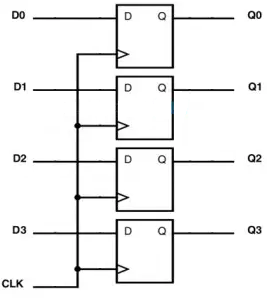
\includegraphics[
                width=\linewidth,
                height=0.65\textheight,
                keepaspectratio
            ]{images/buffer.png}
        \end{column}

    \end{columns}
\end{frame}